\section{Technologies}

\subsection{HTTP and REST}

Hypertext Transfer Protocol is one of the basic protocols of the World Wide Web.

It implements the request-response model, and the client-server model. Take example of user navigation to search engine. In such case, the user's web browser is the \textbf{client}, and the computer where search engine is stored is the \textbf{server}. Typing the URL and hitting return key creates a \textbf{request} which is sent to the server over HTTP. Server processes this request and generates a \textbf{response}. The response is sent back to client (the user's browser) which processes it and presents data to user.

The request message is a short message containing the following: Method, path, headers and optional message body. Before we can discuss REST, it’s important to remind all HTTP methods. (GET and POST are the common ones, because they are supported by all browsers.)

Representational state transfer, or REST, is a style of architecture for HTTP interfaces. It's basic idea is that every object is represented as a resource. Actions can be performed on resources, such as index (will return list of all objects for specific entity), create (will create new record for entity), update (will update parameters of record) and delete (will remove a record). In REST, these actions are mapped to method and URL pairs. \citep{rails_way}

Atmosphere will act as client in the REST architecture. It will expect the source to be a RESTful HTTP interface, but still configurable. 

\subsection{HTML5}

Since Atmosphere relies heavily on HTML5 features, some of them will be described in this section. 

HTML5 is the new version of HTML with support for all kinds of new features. The following sections will go through these features, discuss their use and support in the web browsers. Also, we’ll discuss how these features fit with Atmosphere and what use they can be made of.

Before it would be worth mentioning that by using HTML5 there is increased chance that the application won’t work correctly, or won’t work at all for some users. In a good application, users with old browsers would be informed about this and not allowed to use the application at all, instead of leading them into thinking the issues are caused by the application. 

Can be this problem solved in a more elegant manner? Is there any solution that would bring bring the new features to users with old browsers? That depends on what feature it is. For example, if the browser doesn’t support WebSockets (which is a real situation – Android web browser doesn’t support it.), then the push notifications should be disabled, but the application should work without them. That is of course the case if the application is not completely based on WebSockets. Atmosphere applies this concept of graceful degradation: If the WebSocket support is not present, it simply won’t be used, but the application will still work through the REST interface as normal.

That was an example of degradable feature, there are more fundamental ones that simply require support. In that case there is no other solution than demanding user to upgrade their browser.

Another interesting solution is to bundle the application along with a modern browser and distribute it as a desktop application.

\subsubsection{CSS3}

CSS3 allows advanced styling of interface elements without use of images. The main advantage is being able to change looks later in the development process without having to use an image editor.

\emph{Animations} generally improve user experience by visualizing the action performed by the user. With CSS3, animations can be rendered using JavaScript. That means, instead of computing properties for each frame of animations, it is the responsibility of web browser to render it. Some browsers use GPU to accelerate these animations, which makes the interface feel much more like a native application. 

\emph{Border radius} is a simple feature that allows rendering elements with a border radius. 

\emph{Shadows} allow rendering shadows as if cast by text (text-shadow) or a some element (box-shadow.) 

\emph{Flex box} is a feature for creating „flexible“ boxes, that means making elements automatically expand to some part of the screen. It allows building interfaces, that looks like native user interface instead of web page. The original solution was mostly absolute positioning or JavaScript that would automatically reposition elements whenever the window was resized. 

\emph{Font face} allows using custom fonts and is already widely used. There are services, such as Typekit or Google Web Fonts, that let developers use any font from their collection by simply including short stylesheet in the page. 

\emph{Gradients} allow styling elements with gradients without having to use images.

Atmosphere doesn’t directly require any of these features as it is not working with the interface directly.  

\subsubsection{Geolocation}

Some HTML5 browsers support geolocation – a programming interface that lets web application request current location of the user, after user allows the application to access it. It is easy to gracefuly degrade when this feature is not available.

It is available on most of the mobile devices. 

Atmosphere doesn’t use this feature in any way.

\subsubsection{Canvas}

Canvas is a HTML5 element that allows dynamic rendering of vector objects and bitmaps. It is commonly used in graphic applications.

It is supported in all browsers, except Internet Explorer supports it only from version 9.0.

Atmosphere doesn’t use the canvas element.

\subsubsection{WebGL}

WebGL is a JavaScript extension that allows generation of interactive 3D graphics by sending instructions directly to GPU. It’s based on OpenGL ES 2.0. 

In supported browsers, WebGL is automatically enabled if user hardware is compatible. WebGL is  supported in version 9.0 and newer of Google Chrome, 4.0 and newer of Mozilla Firefox, 5.1 and newer of Safari (altough Safari has WebGL disabled by default.) As of time of writing, it is not supported by Internet Explorer. 

Atmosphere doesn’t use this feature either.

\subsubsection{Audio}

Audio is an element that is used to play sounds in web browsers. Before HTML5, this task was usually handled by embedding Flash file. 

Audio has been around for longer than other features and is currently supported by all major browsers.

\subsubsection{Local Storage}

Local storage is the one feature that used to make desktop application superior to web application in many cases. In the years 2000 to 2009 there have been many attempts to somehow add local storage to web applications. These include userData of Internet Explorer (part of DHTML Behaviors), Local Shared Objects of Adobe Flash and bridges with JavaScript, and SQLite databases provided by Google Gears.

HTML5 brings a new feature, Local Storage or sometimes called Web Storage. Websites can store up to 5MB of data in key/value pairs and even more after demanding user’s permission. Local Storage is supported by all major browsers, including Internet Explorer from version 8.0. It is also supported on mobile browsers, both Android (2.0 and up) and iPhone (2.0 and up.). 

Local Storage is thus a reliable way of storing application data on the client side. Atmosphere uses it to store local objects. 

\subsubsection{WebSQL and IndexedDB}

Simple key value storage is a good solution for simple applications. But sometimes greater flexibility is required. In desktop application such cases usually employ SQLite database, or other SQL based database solution. 

There are two solutions for the web: First one is WebSQL, which is similar to Google Gears a JavaScript interface to SQLite database. Such solution provides enough flexibility to store data in a more sophisticated manner than simple key value storage.

Unfortunately, WebSQL is not supported by Internet Explorer or Mozilla Firefox. This is not a result of slowness in development, Mozilla has stated they are not planning to support WebSQL. \citep{mozilla_indexeddb} Also, in 2010, W3C announced that WebSQL is a deprecated specification. \citep{w3c_webdatabase}

There is another solution, IndexedDB, which differs from WebSQL in API. Instead of writing SQL requests manually, it provides a JavaScript API to manipulate objects. Mozilla has implemented this database in version 4.0 of Firefox, it is also partially supported by Google Chrome 11.

Since not of these database is fully supported, Atmosphere doesn’t use either. Instead, applications should execute complicated database requests on the server and use REST API to retreive a subset of resources relevant to the user thus minimalizing complexity of client-side database requests making key-value storage sufficient.

Client-side SQL databases will be an interesting solution, and as they become a feature that’s supported on all platforms Atmosphere will try to use them. Until then we’ll stick with Local Storage.

\subsubsection{Websockets}

WebSockets is an extension of HTTP protocol. WebSockets hide the low level networking to provide simple API for connecting and sending simple text messages. 

WebSockets are most commonly used in web browsers, but not limited to. There are client libraries in languages such us Objective-C or Java, so they can be used in native iOS or Android applications.

The server part can be written in any language. There are servers written in Ruby, PHP, Java and others. But there is one server side environment that is favorite amongst many developers who use WebSockets. It’s Node.js, the environment that uses JavaScript as server language. Thanks to Node.js it’s possible to write server and client side for WebSockets in the same language with very similar API.  

WebSockets are supported in all current version of browsers. For Atmosphere, that would suffice, because the application can work without WebSockets, it would gracefully degrade to work without notifications. There are of course countless web applications that are based on WebSockets, that couldn’t work without them. There’s a library for this very purpose: Socket.IO. \citep{socketio}

\begin{quotation}
Socket.IO aims to make realtime apps possible in every browser and mobile device, blurring the differences between the different transport mechanisms. It's care-free realtime 100\% in JavaScript. \citep{socketio}
\end{quotation}

The idea behind Socket.IO is to use WebSocket when available and gracefully downgrade to other workarounds for push notifications in the brower. These include Flash file bridged with JavaScript, AJAX long polling and others. To use Socket.IO, a library needs to be included on both client and server side. With Socket.IO library the server side is expected to be written in JavaScript on Node.js, but there are other third party libraries that work in other environments.

Atmosphere uses Socket.IO which allows for notifications to work practically in any browser. (Internet Explorer 5.5+, Safari 3+, Google Chrome 4+, Firefox 3+, Opera 10.61+).

\subsubsection{Cache Manifest (Offline Applications)}

Cache Manifest is a feature that allows accessing a web application without active network connection. In order to implement cache manifest, a list of all resources that application require to work must be create and exposed using the cache manifest API. This will cause browser to store the resources for offline usage.

One of the effects is that the next time the web application is used, these resources will be loaded locally making the web application load instantly.

Using cache manifest also allows web application to be used offline without any internet connection at all. Atmosphere makes this possible by storing all objects locally. When user alters an object, it’s only marked as changed and pushed to the server the next time internet connection is available. 

By using both cache manifest and Atmosphere it’s possible to build web applications that simply work offline. 

\subsubsection{Conclusion}

Features listed here hardly include all of the ever evolving features of HTML5. We focused on the clue feature for Atmosphere, but we mentioned most of the features that could help building a next generation web application.

\subsection{PhoneGap and MacGap}

\begin{quotation}
PhoneGap is an HTML5 app platform that allows you to author native applications with web technologies and get access to APIs and app stores. PhoneGap leverages web technologies developers already know best... HTML and JavaScript. \citep{phonegap}
\end{quotation}

PhoneGap is a platform for wrapping HTML5 application into native packages. MacGap is an extension of PhoneGap that allows doing the same with desktop applications. MacGap works only on Mac computers.  There is a couple of interesting consenquences of using these platforms.

The first one is obvious. PhoneGap allows accessing native features of the device with JavaScript API. This connection is made using bridge between native code and UI element responsible for displaying the web page. (Usually called a WebView.) It’s possible to use some native features, such as accelometer, camera or compass. Lower level features are available too: Files, media, storage, notifications. 

Second is related to the way user perceive software. They are used to web applications being slow, laggy and unresponsive. Native applications, on the other hand, they perceive as fast and easy to use. Today it’s possible to build apps based on HTML5 (if built correctly), that are almost as good as native apps. When users are aware that they are dealing with a web application, not a native one, they expect the application to be slow and unresponsive, like they are used to with almost all web applications. 

Disguising a well-made web application as a native application may result into user believing they’re working with a native app, especially when the user is not too technical.

A great example is recently released LinkedIn iPad application of which 95\% is built with HTML5 instead of native technologies. (Shown in Figure \ref{fig:linkedin}.) \citep{linkedin_ipad}

\begin{figure}[htbp]
  \centering
    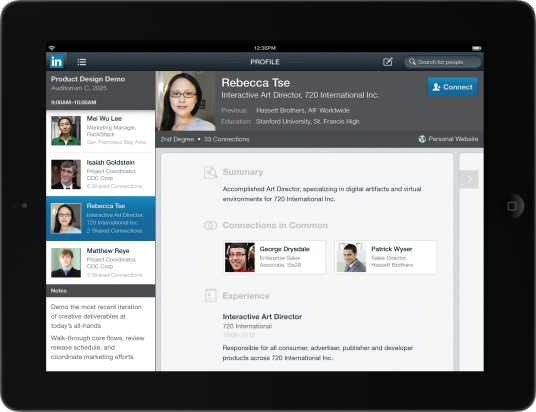
\includegraphics[height=3in]{figures/LinkedIn_iPad.jpg}
  \caption{LinkedIn iPad application}
  \label{fig:linkedin}
\end{figure}

The last reason is the ability to publish application in the App Store or Android Market. For Apple platform, App Store is the only way to distribute software (except for jailbroken devices.) For Android platform, it is possible to install applications from other sources than the Market, but in both cases having an application exposed in the App Store/Market helps uses find it, and increases downloads or sales.

Atmosphere doesn’t use these platforms in a direct way, but developer is encouraged to use them. 

\subsection{Cocoa}

Cocoa is a platform for developing Mac desktop and iOS mobile applications. The implementation of Atmosphere includes libraries for this platform.

Cocoa allows building native application using the Objective-C language and a tool called Interface Builder. This two allow developer to instantiate objects and graphically layout interface elements. All of the objects are then archived, frozen in place. When the interface file is loaded, the contents are unarchived, but not instantiated.

Cocoa provides basic elements to build both desktop and mobile applications. On desktop, forms elements, tables, collections and others are available. Mobile version contains different views made for touch devices. Also, the mobile version is extended by the touch framework for recognizing touch gestures, and other features specific for mobile devices.

Organization of code is usually done within the MVC pattern. For the model layer there is the Core Data library, that acts as peristance framework. The desktop version of Cocoa supports data bindings that automatically upate interfaces elements according to changes to models. This feature significantly reduces glue code in the controllers.

Another  very common pattern used by Cocoa is the observer pattern. There is notification center object, usually one for the application, which any objects can use to subscribe to notifications, or post notifications to. 

Core Data library persists special objects called managed objects into file or a database.  It manages attributes and relations of objects. Core Data uses fixed data schema which can be defined using a file or programatically. This is different from HTML5 as Core Data objects have fixed schema, and HTML5 are just objects serialized into key value storage. With Core Data it is of course possible to write more complicated applications with more complicated requests, because it can use SQLite as storage mechanism.

Atmosphere library sits on top of Core Data and adds automatic networking. Fetching or synchronizing objects can be triggered manually, or by watching  for changes using the notification center. (Observer pattern.)

Cocoa is a very deep framework with many features. This section is just an introduction to basic concepts and features that are later utilized by Atmosphere. 
